\documentclass{beamer}

% import packages
% packages for the poster itself
\usepackage{lmodern}
\usepackage[a0paper]{beamerposter}
\usepackage{graphicx}
\usepackage{booktabs}
\usepackage{tikz}
\usepackage{pgfplots}
\usepackage{anyfontsize}
\usepackage{multicol}
\usepackage{subcaption}
% packages for citations
\usepackage{hyperref}
\usepackage{csquotes}
\usepackage[style=numeric, backend=biber]{biblatex}
% packages for specific content
\usepackage{amsmath}
\usepackage{amsfonts}
\usepackage{amssymb}
\usepackage{amsthm}
\usepackage{siunitx}

% configure pgfplots
\pgfplotsset{compat=1.14}

% specify theme and color theme
\usetheme{gemini}
\usecolortheme{earth}

% load the bibligraphy file
\addbibresource{citations.bib}

% define poster lengths for columns
% If you have N columns, choose \sepwidth and \colwidth such that
% (N+1)*\sepwidth + N*\colwidth = \paperwidth
\newlength{\sepwidth}
\newlength{\colwidth}
\setlength{\sepwidth}{0.025\paperwidth}
\setlength{\colwidth}{0.283\paperwidth}
% define the separator column command
\newcommand{\separatorcolumn}{\begin{column}{\sepwidth}\end{column}}

% configure the author block
\title{The Knitted Torus}
\author{Nicholas Klein \and Calvin Sprouse}
\institute{Department of Mathematics, Central Washington University}

% configure the footer
\footercontent{
MATH 207 Honors Seminar \hfill
2024 May 31
}

% define logo
\logoright{
\includegraphics[height=7cm]{figures/logos/cwu_logo.png}}


%-----------------------------------------------------------------------------%
% begin poster
\begin{document}
% begin the content framework
\begin{frame}[t]
\begin{columns}[t]
\separatorcolumn\separatorcolumn%

%-----------------------------------------------------------------------------%
% first column of content
\begin{column}{\colwidth}
%------------------------------------------------%
% introduction/abstract block
\begin{block}{Introduction}

A torus, not to be confused with Taurus of the Zodiac, is a type of geometry with many familiar real world examples. Some common real world tori are doughnuts, onion rings, grip strength trainers, and gymnastic rings. It should be noted that these are examples of solid tori whereas mathematicians tend to study a hollow torus.

\bigskip
\begin{figure}[htbp]
    \centering
    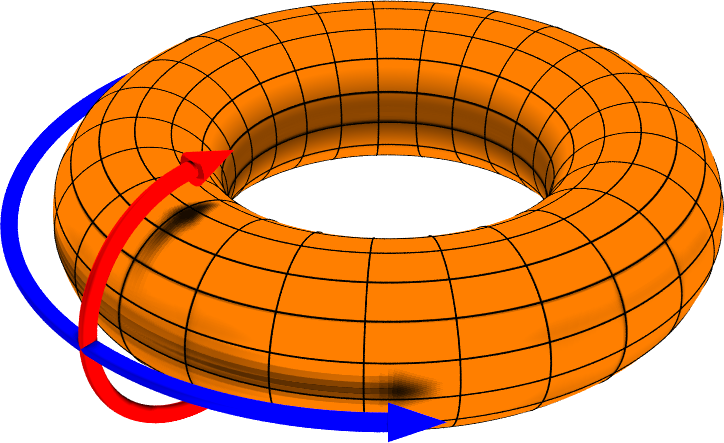
\includegraphics[width=0.5\textwidth]{figures/poloidal.png}
    \caption{The toroidal coordinate system. The blue arrow indicates the toroidal direction and the red arrow indicates the poloidal direction. Figure by DaveBurke, distributed under CC-BY 2.5 license.}
    \label{fig:torus_coords}
\end{figure}

The torus can be parameterized as
\begin{align*}
x(\theta, \phi) &= \left(R + r\cos(\theta)\right)\cos(\phi), \\
y(\theta, \phi) &= \left(R + r\cos(\theta)\right)\sin(\phi), \\
z(\theta, \phi) &= r\sin(\theta),
\end{align*}
where \(\theta,\phi\in\left[0,2\pi\right)\). From Figure~\ref{fig:torus_coords}, the toroidal arrow lies in the \(xy\)-plane. The major radius, \(R\), defines a circle in the toroidal direction and the minor radius, \(r\), defines the poloidal circle. The ratio of the two radii, \(R/r\), is called the aspect ratio.

\bigskip
\begin{figure}[ht]
    \centering
    \begin{minipage}[b]{0.3\textwidth}
        \centering
        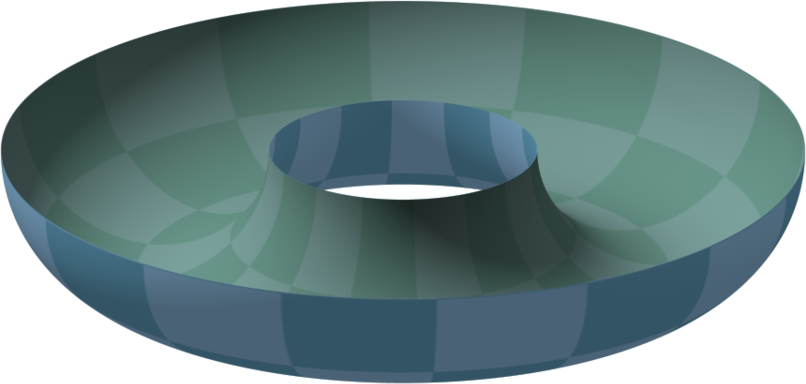
\includegraphics[width=\textwidth]{figures/torus_ring.png}
        \caption*{(a)}
        \label{fig:ring_torus}
    \end{minipage}
    \begin{minipage}[b]{0.3\textwidth}
        \centering
        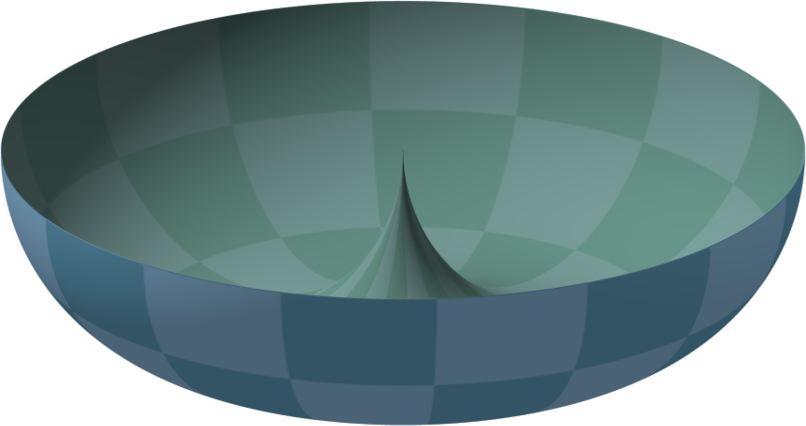
\includegraphics[width=\textwidth]{figures/torus_horn.png}
        \caption*{(b)}
        \label{fig:horn_torus}
    \end{minipage}
    \begin{minipage}[b]{0.3\textwidth}
        \centering
        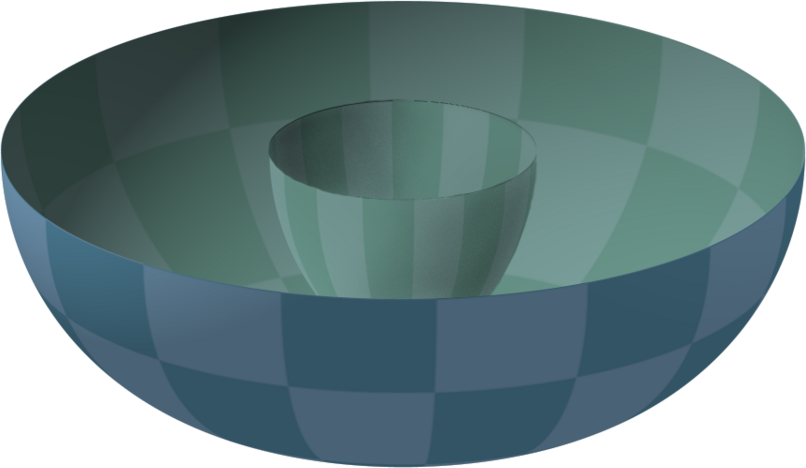
\includegraphics[width=\textwidth]{figures/torus_spindle.png}
        \caption*{(c)}
        \label{fig:spindle_torus}
    \end{minipage}
    \caption{Three different classes of standard tori. The ring torus, (a); the horn torus, (b); and the spindle torus, (c). The spindle torus has two distinct shells. The inner shell is called a lemon and the outer shell is called an apple.}
    \label{fig:three_torus}
\end{figure}

There exist four special classifications of aspect ratio:
\begin{align*}
R>r,&\ \text{the familiar torus sometimes called the ring torus, Figure~\ref{fig:ring_torus};}\\
R=r,&\ \text{the horn torus with a shape similar to an apple, Figure~\ref{fig:horn_torus};}\\
R<r,&\ \text{the spindle torus which self-intersects creating two surfaces, Figure~\ref{fig:spindle_torus};}\\
R=0,&\ \text{the sphere.}
\end{align*}

\begin{figure}
    \centering
    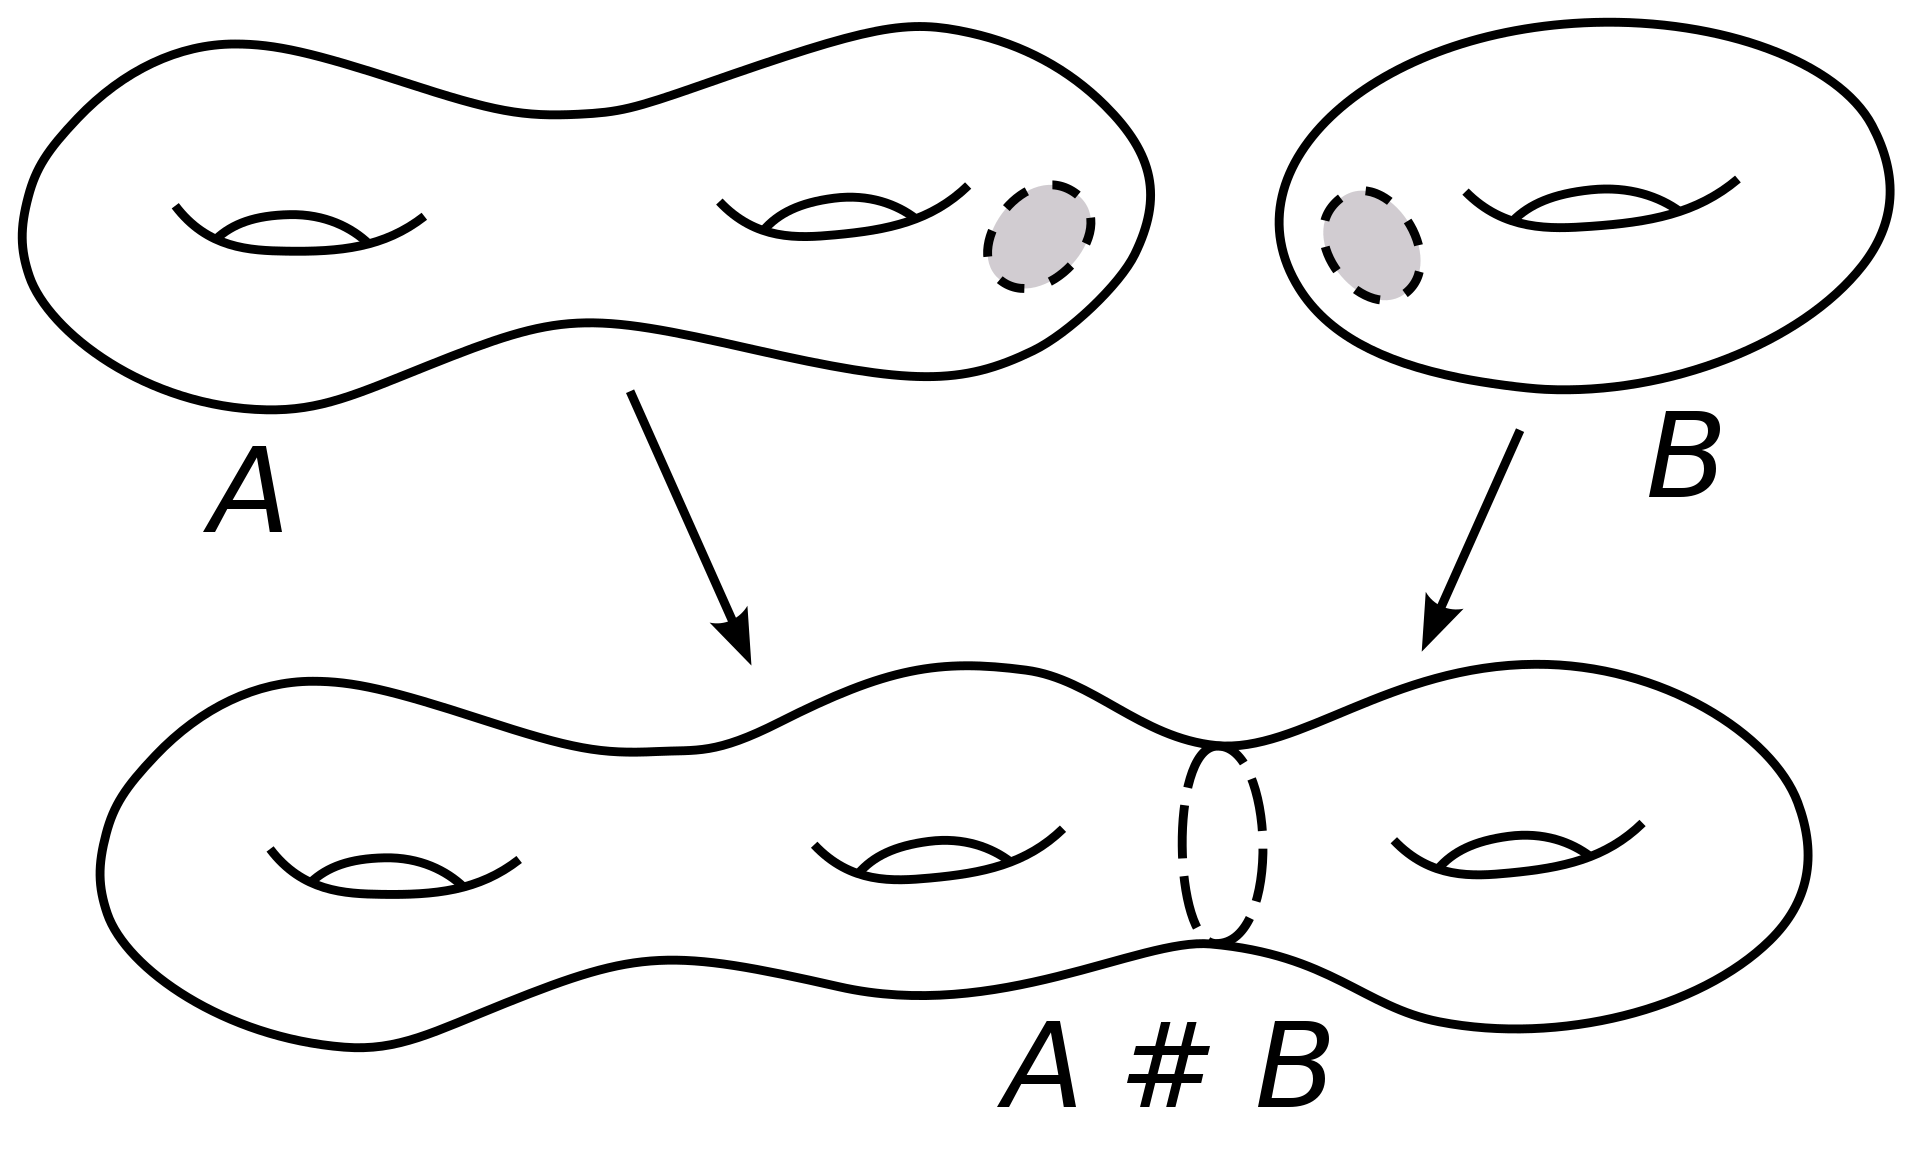
\includegraphics[width=0.7\textwidth]{figures/genus.png}
    \caption{A diagram illustrating the ``gluing together" of tori, resulting in a topological space with a higher genus. Figure by Oleg Alexandrov, distributed under CC-BY 2.5 license.}
    \label{fig:genus}
\end{figure}

\end{block}
\end{column}
\separatorcolumn%

%-----------------------------------------------------------------------------%
% second column of content
\begin{column}{\colwidth}
%------------------------------------------------%
% topological definition of a torus
\begin{block}{Topology}

The torus (or 2-torus) is defined as \( S^1 \times S^1 \), where \(S^1\) is the unit circle. The operation \( \times \) is the Cartesian product, meaning the set \( S^1 \times S^1 \) consists of all ordered pairs \( (x,y) \), where \(x\in S^1\) and \(y\in S^1\) \autocite{morris1989topology}. This can be interpreted as a circle revolved around a circle.

One may also think of the torus as a square where the opposite ends have been glued together, as seen on this poster. This way of thinking of the torus uses the fundamental polygon of the torus, which encodes information about the torus as a topological space.

\begin{figure}
    \centering
    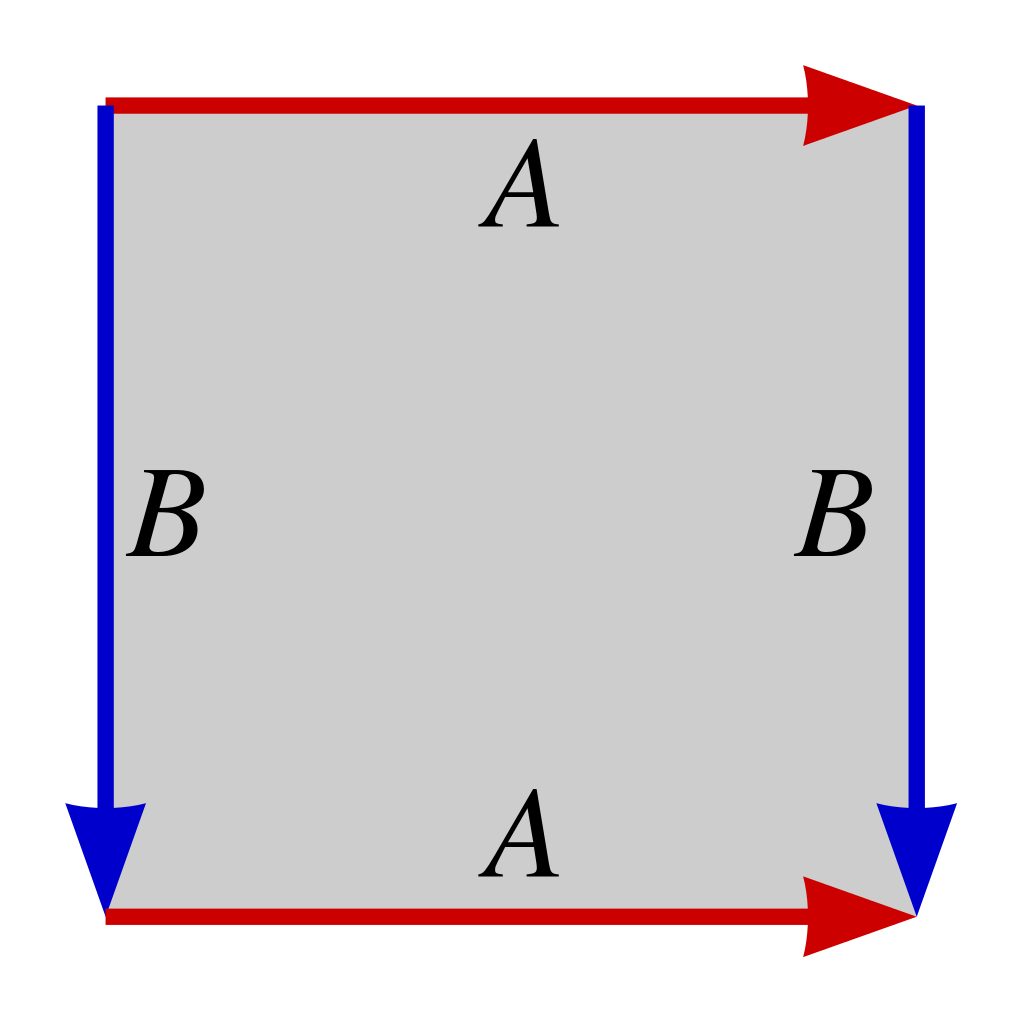
\includegraphics[width=0.4\textwidth]{figures/torus square.png}
    \caption{The fundamental polygon defined for the torus. Figure by Ilmari Karonen, distributed under CC-BY 2.5 license.}
    \label{fig:torus_square}
\end{figure}

A fundamental concept in topology in that of a genus. The genus of a topological space can be thought of as the number of ``holes" in the space. For example, the torus has genus 1, representing the one hole that is in the torus. The technical definition of the genus (which we will not get into here) involves the ``gluing together" of tori!

\bigskip
\begin{figure}[htbp]
    \centering
    \begin{minipage}[b]{0.32\textwidth}
        \centering
        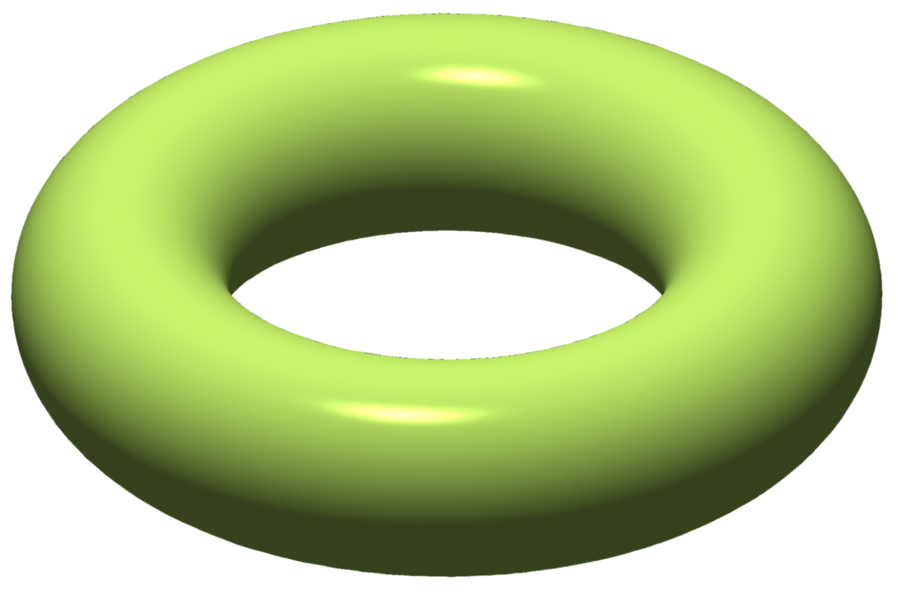
\includegraphics[width=\textwidth]{figures/single_torus.png}
        \caption{A genus one topological space, the familiar torus. Figure by Oleg Alexandrov, distributed under CC-BY 2.5 license.}
        \label{fig:single torus}
    \end{minipage}
    \hfill
    \begin{minipage}[b]{0.32\textwidth}
        \centering
        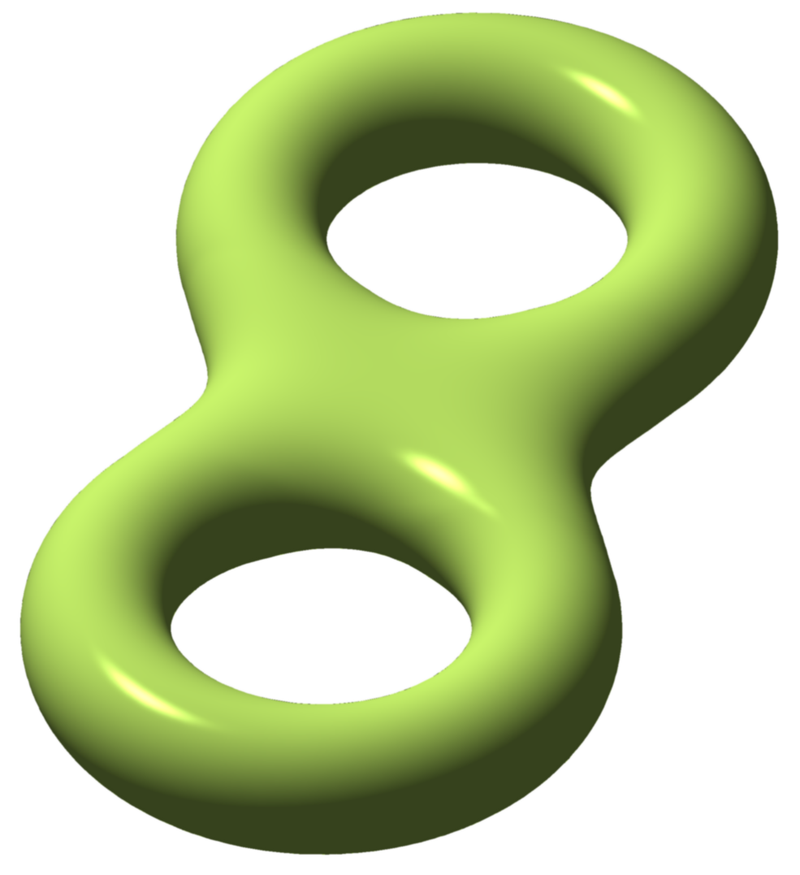
\includegraphics[width=0.7\textwidth]{figures/double_torus.png}
        \caption{A genus two topological space. Figure by Oleg Alexandrov, distributed under CC-BY 2.5 license.}
        \label{fig:double torus}
    \end{minipage}
    \hfill
    \begin{minipage}[b]{0.32\textwidth}
        \centering
        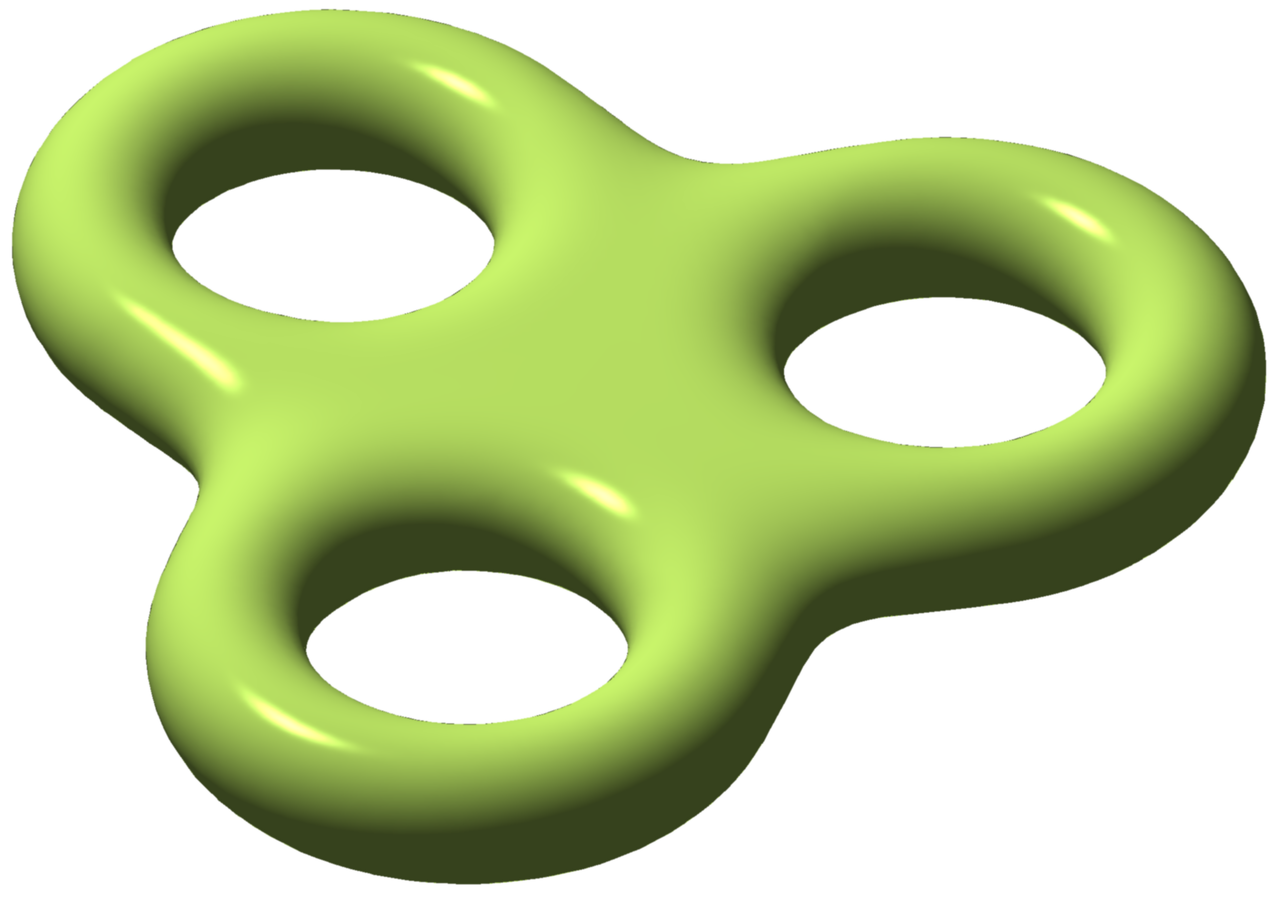
\includegraphics[width=\textwidth]{figures/triple_torus.png}
        \caption{A genus three topological space. Figure by Oleg Alexandrov, distributed under CC-BY 2.5 license.}
        \label{fig:triple torus}
    \end{minipage}

\end{figure}

A topological property that the torus processes is that of connectedness. A topological space is connected if it not disconnected. That is, the space cannot be written as the union of two sets with no overlap. An informal way of thinking about this property is that from any point in the topological space, it is possible to get to any other point in that space while staying completely inside that space. On the surface of a torus, it possible to go to any other point by moving along the torus, and so the torus is connected.

Another topological property that the torus processes is that of compactness. In order for a topological space to be compact, it must contain all of it's limiting values. For example, the interval \([0,1]\) is compact, but \((0,1)\) is not compact because 0 and 1 are not included. All limiting values of points on the torus are contained on the surface of the torus, and so the torus is compact. 

These two topological properties along with the fact that the torus does not have a boundary (meaning you can move along the torus in a single direction forever without leaving the surface of the torus) make the torus a closed surface!
\end{block}
\end{column}
\separatorcolumn%

%-----------------------------------------------------------------------------%
% third column of content
\begin{column}{\colwidth}
%------------------------------------------------%
% applying the torus to math and other stystems
\begin{block}{Tori in Nature}

We have created a knitted torus based on a pattern generated by Ref.\autocite{szczepanski_knitted_nodate}. Our knitted torus, tori if all went well, are meant to represent ring torus of outer radius 4 inches and inner radius 1 inch. These measurements translate to a minor radius of \(r=1.5\,\text{in}\) and major radius \(R=3.5\,\text{in}\) for a torus of aspect ratio of \(7/3\). 

A fun idea is that the potential shape of our universe is that of a torus! While this probably isn't the case, there are some good reasons why one might consider the torus as the shape of our universe. Some evidence comes in the form of the cosmic microwave background (CMB). This first light of the universe indicates connectedness not captured by the most accepted geometry of the universe~\autocite{aurich_variance_2021}.

% \begin{figure}
%     \centering
%     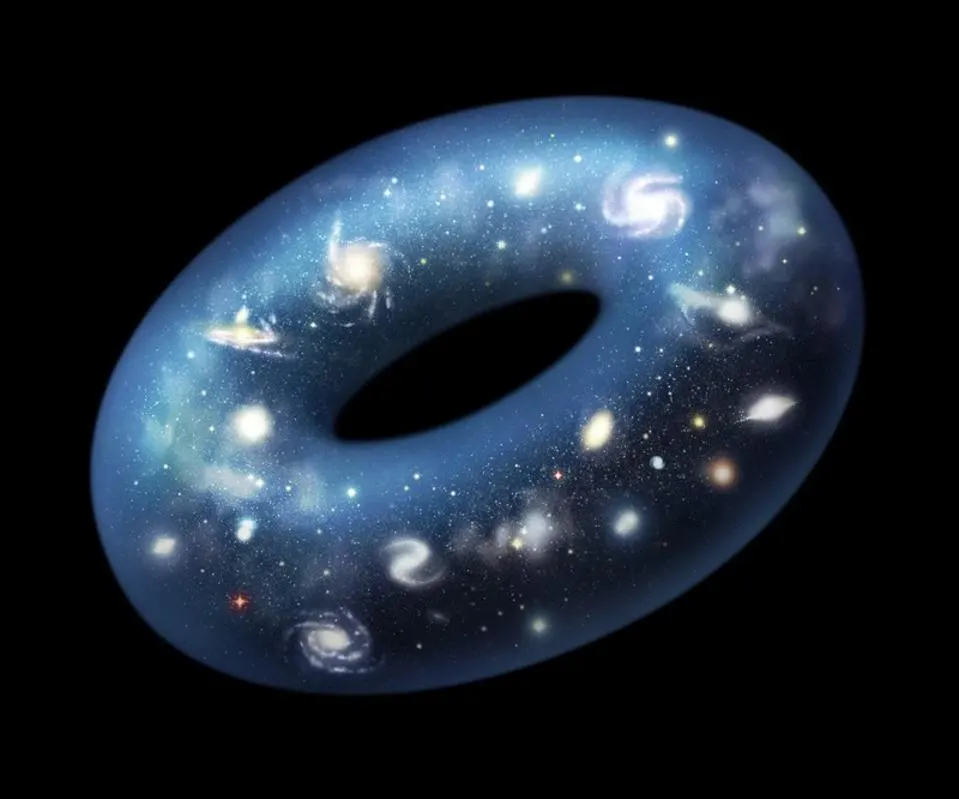
\includegraphics[width=0.6\textwidth]{figures/torus universe.png}
%     \caption{The universe depicted on a torus. Image obtained from the Forbes article \textit{Why The Universe Probably Isn’t Shaped Like A Donut} by Ethan Siegel}
%     \label{fig:torus universe}
% \end{figure}

The torus is also the geometry of choice for those looking to harness the power of nuclear fusion.

\begin{figure}
    \centering
    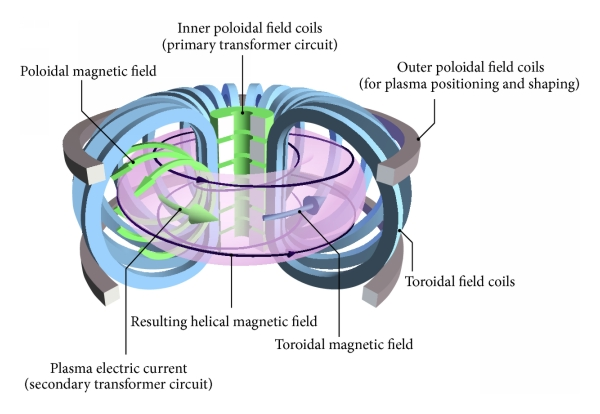
\includegraphics[width=0.8\textwidth]{figures/tokomak.jpg}
    \caption{The magnetic fields created in a tokomak nuclear fusion reactor. Running in the toroidal direction, and shown in blue, are magnetic fields used to swirl and contain the plasma. Poloidal fields are used to fine shape the plasma. The combination of toroidal and poloidal fields is shown as the helical magnetic field in pink. Figure from Ref.~\autocite{li_optimal_2014}}.
    \label{fig:tokomak}
\end{figure}

In nuclear fusion, the torus is chosen because it permits a plasma to be in constant motion without requiring an infinitely long chamber.
\bigskip


\end{block}
%------------------------------------------------%
% reference block
\begin{block}{References}
\nocite{morris1989topology, ding_author_2024}
\printbibliography

\end{block}
\end{column}
\separatorcolumn\separatorcolumn%

\end{columns}
\end{frame}
\end{document}
